\chapter{关联之HBT}
\section{干涉学介绍}
HBT首先利用两个光子之间的关联来确定实验源和天体源的角径。%
由于这种关联与同时存在两个时空点上测得的两粒子强度有关,%
故而称为强度干涉学,%
也称为HBT关联。%
人们发现在不同的能区中HBT半径随横动量增大而减小这一非常一致的趋势,%
这体现了发射原的横向和纵向的膨胀性。%
\par
人们认为在RHIC能区最高能量的碰撞下会发生从强子气体到部分子的转变。%
流体力学预言如果出现QGP,%
粒子发射原的寿命会变长,%
空间尺度会变大,%
从而导致HBT半径增大,%
而RHIC的实验结果并没有看到这样的相变信号。%
S. Pratt在流体力学模型框架下,%
通过综合的考虑初始条件、态方程、粘滞性对HBT半径的影响,%
发现HBT之谜也可以在流体力学模型的框架下得到解决。%
\par
强度干涉学的基本思想来源于使得波函数产生对称性的粒子全同原理。%
具体地说,就是要描述两个全同的玻色子的波函数要满足交换对称性,%
这就导致两粒子在小动量差附近被加强,%
而且这种加强于两粒子的空间分布直接相关。%
{\color{red}{所以,可以利用两粒子动量空间的关联函数来得到坐标空间的信息。}}%

\section{关联函数}
两个全同玻色子关联函数定义为:
\begin{equation}
  \label{eq:chapterSix1}
  C(p_{1}, p_{2}) = N\frac{P_{2}(\textbf{p}_{1}, \textbf{p}_{2})}{P_{1}(\textbf{p}_{1})P_{2}(\textbf{p}_{2})}
\end{equation}
其中,N表示归一化系数,%
$P_{x}(\textbf{p}_{x})$和$P_{2}(\textbf{p}_{1}, \textbf{p}_{2})$分别为单粒子谱和两粒子谱。%
粒子谱的定义为:
\begin{equation}
  \label{eq:chapterSix2}
  P(\textbf{p}) = \int{d^{4}xS(x,p)}
\end{equation}
$S(x,p)$为源函数。%
通过质壳关系和平滑近似我们可以得到:
\begin{equation}
  \label{eq:chapterSix3}
  C(\textbf{q, K}) - 1 = \frac{|\int{d^{4}S(x, K)e^{iqx}}|}{|\int{d^{4}xS(x, K)}|}
\end{equation}
其中,$<...>$表示对发射函数取平均,%
$q=p_{1}-p_{2}$和$K=(p_{1}+p_{2})/2$分别为两粒子的动量差和动量和。%
由于两粒子关联函数只有3个独立变量,%
而发射函数的时空分量包括四个变量(x, t)。%
因此要从关联函数C(q, K)得到S(x, K)必须要包含一定的模型假设。%
利用所谓的\textquotedblleft{归一化相对距离分布}]\textquotedblright{}:
\begin{gather}
  \label{eq:chapterSix4}
  d(x, K) = \int{d^{4}Xs(X+\frac{x}{2}, K)(X-\frac{x}{2}, K)}\\
  s(x, K) = \frac{S(x, K)}{\int{d^{4}xS(x, K)}}
\end{gather}
其中s(x, K)为归一化发射函数。%
由于d(x, K)为偶函数,利用质壳关系,%
关联函数可以写成:
\begin{equation}
  \label{eq:chapterSix5}
  C(q, K) -1 \int{d^{4}cos(q, x)}\int{dtd(x+\beta{t}, t; K)}
\end{equation}
由此,我们可以通过关联函数反推从而得到源函数。%
{\color{red}{在实际过程中,人们并不是直接由关联函数出发重构反射源,%
    而是先对反射函数时空结构进行一定的假设,%
    找到其与HBT之间的关联关系,%
    再反推回到发射源的时空信息。
  }}
\par
高斯参数化是现阶段研究强度干涉学最主要的参数化公式。%
在高能重离子碰撞过程中产生的源具有膨胀性,%
在我们的认知中只有高斯形式能描述这种性质,%
因此就有必要来了解关联函数共和HBT半径的高斯参数化。%
选择合适的关联发射函数带入公式中,%
我们可以得到高斯形式的关联函数:
\begin{equation}
  \label{eq:chapterSix6}
  C(q, K) - 1 = exp[-q_{u}q_{v}\left< \widetilde{x}^{u}\widetilde{x}^{v}(K)\right>]
\end{equation}
其中$\widetilde{x}$定义为时空点x相对于\textquotedblleft{有效发射中心}\textquotedblright{}的距离。%
一般来说根据公式\ref{eq:chapterSix4}
得到的两粒子的平均动量\textbf{K}反应的半宽并不是真正源的大小。%
只有当反射源没有空间动量关联,即$S(x, K) = f(x)g(x)$时得到的半宽才和源真正的半宽是一致的。%
受到质壳关系的限制,%
目前人们采用如下图的方式定义的高斯参数化得到\textquotedblleft{out-side-long}(osl)\textquotedblright{}坐标系:%
long方向与入射方向平行,%
out方向与K的横向分量平行,%
side方向垂直于out,long,%
并且给出了相对动量差q的三个高斯分量$q_{out}, q_{side}, q_{long}$。
\begin{figure}[hbtp]
  \centering
  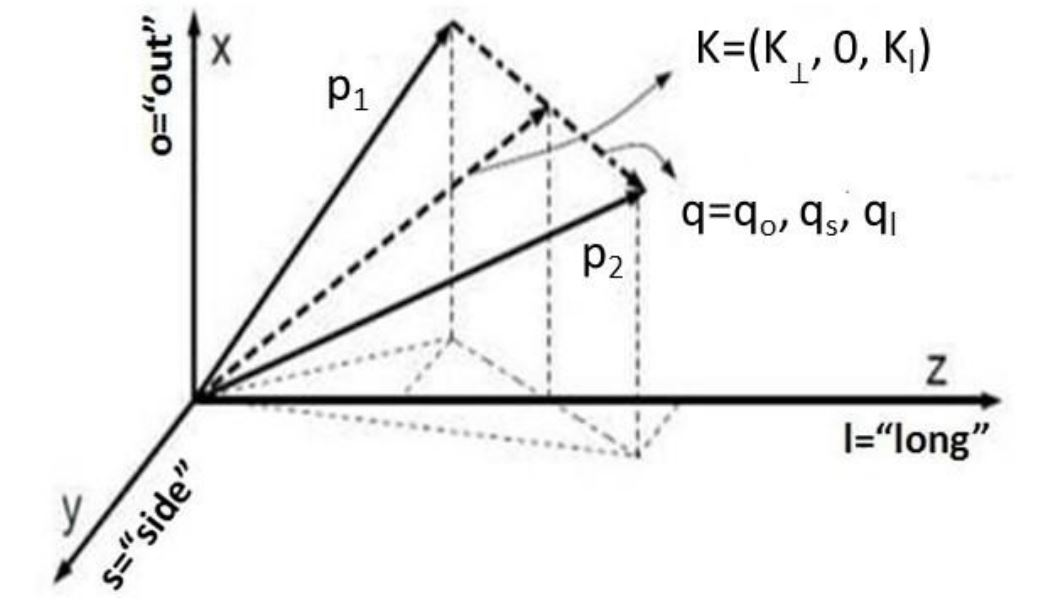
\includegraphics[width=0.8\textwidth]{./chapter06/images/hbt}
  \caption{out-side-long坐标系,其中纵向(long)沿着入射方向。}
  \label{fig:hbt-coordinate}
\end{figure}
在\textquotedblleft{out-side-long(osl)}\textquotedblright{}坐标系中,%
粒子对的时间分量通过质量约束可以忽略,从而得到关联函数的高斯参数化形式:%
\begin{equation}
  \label{eq:chapterSix7}
  C(q, K) - 1 = exp[-\sum_{i,j=o,s,l}R_{ij}^{2}(K)q_{i}q_{j}]
\end{equation}
其中$R_{ij}^{2}(K)q_{i}q_{j}$的六个独立分量称为\textquotedblleft{HBT}\textquotedblright{}半径,%
其形式可以写为:
\begin{equation}
  \label{eq:chapterSix7}
  R_{ij}^{2}(K)q_{i}q_{j} = \left<(\widetilde{x_{i}}-\beta_{i}\widetilde{t_{i}})(\widetilde{x_{j}}-\beta_{j}\widetilde{t_{j}})\right>    \hspace{1cm} i, j = o, s, l
\end{equation}
一般来说,C(q, K)不仅依赖与粒子对平均动量K的横向分量$K_{\perp}$和纵向分量$K_{l}$而且还依赖于横向动量$K_{\perp}$与横向平面的夹角$\Phi$.%
再对心碰撞中(b\~{}0)和LCMS(longitudinally comoving system, $K_{l}=0$)坐标系中,%
会使交叉项消失,从而可以得到:%
\begin{gather}
  R_{s}^{2}(K) = \left< \widetilde{x_{s}}^{2}\right>(K) \\
  R_{o}^{2}(K) = \left< (\widetilde{x_{l}}-\beta_{o}\widetilde{t})^{2} \right>(K) \\
  R_{l}^{2}(K) = \left< \widetilde{x_{l}}^{2} \right>(K)
\end{gather}

\section{高斯热源模拟}
由于高斯热源模型本身假定热源中粒子向外发射是各向同性的,%
而在火球产生之初粒子数在坐标空间沿各个方向分布应该是由中心向边缘递减,%
因此假定为高斯分布。%
在高斯热源模型中,粒子在坐标空间满足高斯分布:%
\begin{equation}
  \label{eq:chapterSix8}
  f(r) = Ar^{2}exp(-\frac{r^{2}}{2R^{2}})
\end{equation}
其中A为归一化常数,R、r均为四维时空方差,%
表示高斯热源在时空上的大小。
\par
通过分析静态高斯热源的时空分布和动量分布,%
我们对高斯热源的HBT关联进行分析。%
这里我们要用到分析HBT关联函数常用的三维拟合公式,%
这个公式要用到前边所推导出的高斯参数化:
\begin{equation}
  \label{eq:chapterSix9}
  C(q, K) = 1 + \lambda exp(-R_{side}^{2}q_{side}^{2} - R_{out}^{2}q_{out}^{2} - R_{long}^{2}q_{long}^{2})
\end{equation}
其中,$q_{long}$是沿粒子入射方向的动量差。

\section{原理}
a schematic is shown of the HBT intensity interferometer.%
Here, waves emitted from sources \textbf{a} and \textbf{b} impinge on detectors \textbf{1} and \textbf{2}.%
The resulting amplitudes seen at each detector are given by:%
\begin{gather}
  A_{1} = \frac{1}{L}(\alpha e^{i(pr_{1a}+\phi_{a})} + \beta e^{i(pr_{1b}+\phi_{b})}) \\
  A_{2} = \frac{1}{L}(\alpha e^{i(pr_{2a}+\phi_{a})} + \beta e^{i(pr_{2b}+\phi_{b})})
\end{gather}
其中$\alpha$和$\beta$ represent the emission strengths at source points \textbf{a} and \textbf{b},%
respectively, and $\phi_{a}$ and $\phi_{b}$ are the starting phases of the two waves as they are emitted from the two source points.%
In this example, both waves are assumed to have been emitted with the same momentum $p$.
\par
The difference between Michelson and HBT interferometry comes about in how the intensities measured at detectors \textbf{1} and \textbf{2}:
\begin{gather}
  I_{1} = |{A_{1}}|^{2} = \frac{1}{L^{2}}(|\alpha |^{2} + |\beta |^{2} + 2\Re[\alpha * \beta e^{i[p(r_{1b}-r_{1a})+(\phi_{b}-\phi_{a})]}]) \\
  I_{2} = |{A_{2}}|^{2} = \frac{1}{L^{2}}(|\alpha |^{2} + |\beta |^{2} + 2\Re[\alpha * \beta e^{i[p(r_{2b}-r_{2a})+(\phi_{b}-\phi_{a})]}]) \\
\end{gather}
are used in the experiment.%
If the intensity is examined for a short time,%
the initial interference pattern will show itself due to the phase variation in the last term of equation.%
If the intensity is averaged over long times,%
these phases cancel due the randomness in $\phi_{a}$ and $\phi_{b}$,%
and the interference fringes seen at the single detectors vanish:
\begin{equation}
  \label{eq:chapterSix10}
  \left<I_{1}\right> = \left<I_{2}\right> = \frac{1}{L^{2}}(|\alpha|^{2} + |\beta|^{2})
\end{equation}
Examination of the coincidence rate, $\left<I_{1}I_{2}\right>$, again averaged over long times,%
gives the product of the two single intensity measurements at the two detectors,%
plus an extra term which depends on the physical extent of the source.%
Normalizing the coincidence rate by the product of the single intensities gives the correlation function,%
a direct link between the property of the source that is to be measured, namely its physical extent,%
and the observed data, or the measured intensities at two detectors:
\begin{equation}
  \label{eq:chapterSix11}
  C(\vec{R}, \vec{d}) = \frac{\left<I_{1}I_{2}\right>}{\left<I_{1}\right>\left<I_{2}\right>} = 1 + \frac{2|\alpha|^{2}|\beta|^{2}}{(|\alpha|^{2}+|\beta|^{2})^{2}}cos[p(r_{1a}-r_{2a}-r_{1b}+r_{2b})]
\end{equation}
Equation \ref{eq:chapterSix11} demonstates that correlations still exist even in time-averaged intensity measurements.%
Although this would prove useful in the astronomical measurements made by Hanbury Brown and Twiss,%
its most consequential impact would be in the realm of particle physics.%
Eventually, techniques were developed that allowed the amplitudes from widely spaced radio telescopes to be
combined without loss of phase information,%
and Michelson interferometry soon emerged again as the primary method of determining angular diameters of stellar objects.

\section{Theory of Identical Boson Interferometry}
Pions emitted from a heavy-ion collision behave according to the QED equation of state for free-traveling particle, the Klein-Gordon equation:
\begin{equation}
  \label{eq:chapterSix12}
  \left(\frac{\partial^{2}}{\partial{t^{2}}} + \nabla^{2} + m_{\pi}^{2}\right)\Phi(x) = J(x)
\end{equation}
In this equation, J(x) represents the nuclear current operator acting as the source of pions,%
$m_{\pi}$ is the mass of a pion and $\Phi(x)$ is the pion field.%

\section{Pion field Operators}
The single and two-particle coincidence momentum probability distributions for pions are given below:
\begin{gather}
  \label{eq:chapterSix15}
  P_{1}(p) = E_{p}\frac{dN}{d^{3}p} = E_{p}\left<a_{p}^{+}a_{p}\right> \\
  P_{2}(p_{1}, p_{2}) = E_{p_{1}}E_{p_{2}}\frac{dN}{d^{3}p_{1}d^{3}p_{2}} = E_{p_{1}}E_{p_{2}}\left<a_{p_{1}}^{+}a_{p_{2}}^{+}a_{p_{2}}a_{p_{1}}\right>
\end{gather}
In the above equation, $E_{p}$ is the energy of a pion with momentum p,%
and $a_{p}^{+}, a_{p}$ represent the creation adn annihilation operators acting on a coherent state $|J>$,%
the solution to equation \ref{eq:chapterSix12}.%
One of the properties of $|J>$ is that it is an eigenstate of $a_{p}$,%
so that
\begin{equation}
  \label{eq:chapterSix13}
  a_{p}|J> = iJ(p)|J>
\end{equation}
equation \ref{eq:chapterSix13} allows an immediate computation of the probability distributions in equation
\ref{eq:chapterSix12}. %
The two-pion correlation function $C(p_{1}, p_{2})$ is the experimentally measured ratio of the two-pion coincidence momentum distribution to the single pion distribution,%
and for the above coherent state |j> it is found to be:
\begin{equation}
  \label{eq:chapterSix14}
  C(p_{1}, p_{2}) = \frac{P_{2}(p_{1}, p_{2})}{P_{1}(p_{1})P_{2}(p_{2})} = \frac{\left< a_{p_{1}}^{+}a_{p_{2}}^{+}a_{p_{2}}a_{p_{1}}\right>}{\left<a_{p_{1}}^{+}a_{p_{1}}\right>\left<a_{p_{2}}^{+}a_{p_{2}}\right>} = \frac{|J(p_{1})|^{2}|J(p_{2})|^{2}}{|J(p_{1})|^{2}|J(p_{2})|^{2}} = 1
\end{equation}
\par
Thus, for pions behaving under the nuclear current operator in equation (\ref{eq:chapterSix12}),%
there are no momentum correlations between pairs.%
In order to calculate the effect of pions emitted from a chaotic source,%
it is necessary to use superposition of classical sources distributed in phase space.%
By averaging over these sources, the two-particle momentum probability distribution (Equation \ref{eq:chapterSix15}) can be factorized as:
\begin{equation}
  \label{eq:chapterSix16}
  P_{2}(p_{1}, p_{2}) = E_{p_{1}}E_{p_{2}}\left<a_{p_{1}}^{+}a_{p_{2}}^{+}a_{p_{2}}a_{p_{1}}\right> = E_{p_{1}}E_{p_{2}}\left[\left<a_{p_{1}}^{+}a_{p_{1}}\right> \left<a_{p_{2}}^{+}a_{p_{2}}\right> + \left<a_{p_{1}}^{+}a_{p_{2}}\right> \left<a_{p_{2}}^{+}a_{p_{1}}\right> \right]
\end{equation}
This factorization assumes independent particle emission, or full sources chaoticity. %
It is one of the central assumptions of HBT.%
Another name for the factorization in equation (\ref{eq:chapterSix16}) is the generalized Wick Theorem.%
Heuristically it can be seen as a description of the two possible paths two identical particles can take after
being emitted from two source points and arriving at two detection points.%
\par
Using equation (\ref{eq:chapterSix16}), the two-pion correlation function can be calculated for a chaotic source:
\begin{equation}
  \label{eq:chapterSix17}
  C_{2}(p_{1}, p_{2}) = \frac{P_{2}(p_{1}, p_{2})}{P_{1}(p_{1})P_{1}(p_{2})} = 1 + \frac{|\left<a_{p_{1}}^{+}a_{p_{2}}\right>|^{2}}{\left<a_{p_{1}}^{+}a_{p_{}}\right>\left<a_{p_{2}}^{+}a_{p_{2}}\right>}
\end{equation}
The expectation values van be computed and related to the Wigner phase-space density,%
S(x, K),%
the quantum mechanical analogue of the classical phase-space density which is a function of both space x and total momentum K.%
The resulting expression is :
\begin{equation}
  \label{eq:chapterSix18}
  \sqrt{E_{p_{i}}E_{p_{j}}}\left<a_{p_{i}}^{+}a_{p_{j}}\right> = \int{S(x, K_{ij})e^{iq_{ij}x}d^{4}x}
\end{equation}
In this equation, $K_{ij} = \frac{p_{i}+p_{j}}{2}$ is the average momentum of a pair of pions i and j,%
and $q_{ij} = |p_{i} - p_{j}|$ is the invariant momentum difference of the pairs.%
Using equation (\ref{eq:chapterSix17}) and (\ref{eq:chapterSix18}) gives the expression for the two-pion correlation function in terms of the Wigner phase-space density:
\begin{equation}
  \label{eq:chapterSix19}
  C_{2}(p_{1}, p_{2}) = 1 + \frac{|\int{d^{4}xS(x,K)e^{iq\cdot{x}}}|^{2}}{\int{d^{4}xS(x, p_{1})}\int{d^{4}xS(x,p_{2})}}
\end{equation}
In order to parameterize the two-pion correlation function in terms of the physical observable of pion momenta,%
the Wigner phase-space emission function $S(x,K)$ can be approximated by a Gaussian distribution.%
This results in a Gaussian correlation function in terms of the momentum difference $q = p_{1} - p_{2}$:
\begin{equation}
  \label{eq:chapterSix20}
  C_{2}(\textbf{q}, \textbf{K}) = 1 + e^{-q_{u}q_{v}\left<\widehat{x}^{u}\widehat{x}^{v}\right>(\textbf{K})}
\end{equation}
其中,$\widetilde{x}^{u}$ describes the rms widths of effect sources of particles with total momentum \textbf{K}. Different parameterizations can obtain these widths in a particular coordinate system to describe the size of the freeze-out region,%
however the widths obtained only describe the length of a \textquotedblleft{region of homogeneity}\textquotedblright where particle pairs with momentum \textbf{K} are emitted.%

\section{Correlation function parameterizations $Q_{inv}$}
The simplest Gaussian parameterization folds all length and time information into one length scale,%
extracted from a distribution of invariant four-momentum differences
\begin{equation}
  \label{eq:chapterSix21}
  Q_{inv} = \sqrt{|p_{1}-p_{2}|^{2} - (E_{1}-E_{2})^{2}}.
\end{equation}
Once the correlation function has been computed,%
it is fit to the following equation:
\begin{equation}
  \label{eq:chapterSix22}
  C_{2}(q, K) = 1 + \lambda(K)e^{-Q_{inv}^{2}\cdot R_{inv}^{2}(K)}
\end{equation}
The $\lambda$ parameter in equation (\ref{eq:chapterSix22}) represents the degree of contamination in the particle sample being studied,%
as well as a measure of the degree of chaoticity in the system.%
In a pure particle sample with ful chaoticity its value would be unity.%
Since the correlation function is one-dimensional, very few statistics are needed to obtain a high quality fit to the data,%
however since the fit parameter $R_{inv}(K)$ folds so much information into one variable,%
it is difficult draw a substantial conclusion about the properties of the source.

\section{Pratt and Bertsch 参数化}
A 3-dimensional cartesian parameterization, first used by S. Pratt and G. Bertsch,%
uses a coordinate system based on the pair momentum \textbf{k}.%
看下图\ref{fig:pratt-coordinate}, for every pair,%
\begin{figure}[hbpt]
  \centering
  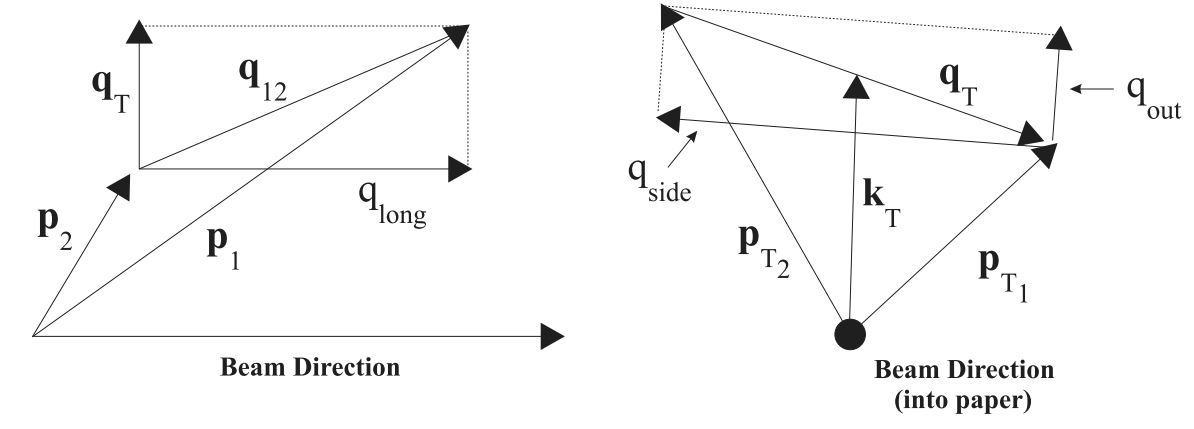
\includegraphics[width=0.8\textwidth]{./chapter06/images/pratt-coordinate}
  \caption{Bertsch-Pratt or cartesian parameterization of the two-pion correlation function.}
  \label{fig:pratt-coordinate}
\end{figure}
The transverse momenta are further split into two components,%
one in the direction of pair and the other in the orthogonal direction.%
From these projections, the invariant momentum difference is calculated for each direction:%
$k_{T}$ (out); $\perp$ to $k_{T}$ (side); and parallel to the beam (long).%
These qualities are then used to produce a 3-dimension correlation function,%
which can be fit to:
\begin{equation}
  \label{eq:chapterSix23}
  C_{2}(q, K) = 1 + \lambda(K)e^{-q_{out}^{2}\cdot R_{out}^{2}(K)-q_{side}^{2}\cdot R_{side}^{2}(K)-q_{long}^{2}\cdot R_{long}^{2}(K)}
\end{equation}
Although all three radius parameters describe lengths of homogeneity along the three axes,%
$R_{out}(K)$ contains additional information about the lifetime of the source,%
due to the fact that this parameter is sensitive to pions which are created at a later time,%
traveling in the direction of \textbf{k} of the pion pair,%
where $R_{side}(\textbf{K})$ is sensitive only to those pions created at the periphery of the freeze-out region,%
at the onset of hadronization, and not to those created at later time.
\par
The difference in sensitivity between $R_{out}(K)$ and $R_{side}(K)$ to the pions with delayed emission allows
in a simplified picture for an estimate of the lifetime of the freeze-out source
\begin{equation}
  \label{eq:chapterSix24}
  R_{out}^{2}(K) - R_{side}^{2}(K) \approx \beta_{\perp}^{2}\left< \widetilde{t}^{2}\right>.
\end{equation}
In this equation, $\beta_{\perp}^{2}$ is the transverse velocity of pair,%
and $\left< \widetilde{t}^{2}\right>$ is the average emission duration of the source.%
Estimating the lifetime with equation (\ref{eq:chapterSix24}) assumes that $R_{out}(K)$ and $R_{side}(K)$ measure approximately the same physical homogeneity length of the source.%
This can be a faulty assumption if the source is opaque, 见下图\ref{fig:opaque-source}
\begin{figure}[hbpt]
  \centering
  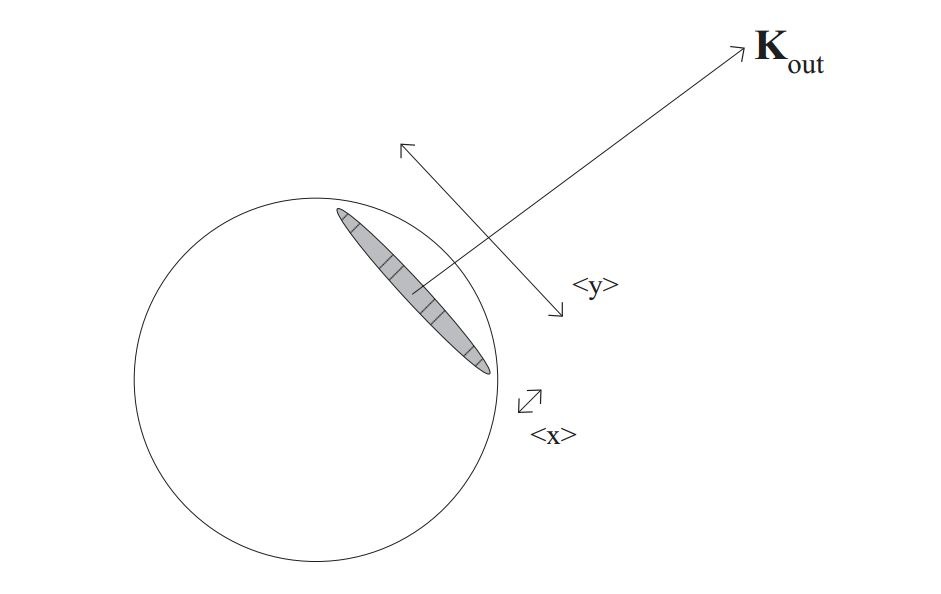
\includegraphics[width=0.8\textwidth]{./chapter06/images/opaque-source}
  \caption{Opaque source, in which $R_{side}$ measures the homogeneity length of the source, but $R_{out}$ is sensitive only to the surface thickness, denoted by $\left< x \right>$.}
  \label{fig:opaque-source}
\end{figure}
in which case $R_{side}(\textbf{K})$ would measure a much larger homogeneity length than $R_{out}(K)$,%
resulting in an imaginary emission lifetime.






%%% Local Variables:
%%% mode: latex
%%% TeX-master: "chapter06"
%%% End:
